\section{Efficient Semantic Parsing}
\label{sec:parsing}
In this section we explain our algorithms and heuristics for efficient semantic
parsing with as little non-determinism as possible, and reducing time complexity
of our parsing strategies.

\subsection{Syntactic-Semantic Parsing}
If using a naïve strategy on the trees yields an exponential algorithm,
the best way to improve the algorithm, is to directly leave the naïve strategy.
To do so, we could simply extend the grammar system used to do the syntactic
part of the parsing.
In this section, we will take the example of a CFG since it suffices to create
our typing combinators,
For example, we can increase the alphabet to be the free monoid on the product
$\Sigma$ of the usual base alphabet and $\bar{\mC}$ our typing category.
Since the usual syntactic structure and our combination modes can both be
expressed by CFGs (or almost, cf Figure \ref{fig:combination-cfg}), our product
system can be expressed by (almost) a CFG.
Here, we change our notations from the proof trees of Figure
\ref{tab:proof-trees} to have a more explicit grammar of combination modes
provided below is a rewriting of the proof trees provided earlier, and
highlights the combination modes in a simpler way, based on
\cite{bumfordEffectdrivenInterpretationFunctors2025} as it simplifies the
rewriting of our typing judgements in a CFG\footnote{That, in a sense, was
	already implicitly provided in Figure \ref{tab:judgements}.}.
The grammars provided  in Figures \ref{fig:english-cfg} and \ref{fig:combination-cfg}
are actually used from right to left, as we actually do combinations over the
types and syntactic categories of the words and try to reduce the sentence, not
derive it from nothing.
Now, all the improvements discussed in Section \ref{subsec:rewrite}
can still be applied here, just a bit differently, as this amounts to reducing
ambiguity in the grammar.

\begin{figure}
	\centering
	{\centering
\setlength{\columnsep}{-1.5cm}
\begin{multicols}{2}
	\def\arraystretch{1.2}
	\begin{mgrammar}
		\gskip
		\firstrule{>, b}{\left(a\to b\right), a}{}
		\firstrule{<, b}{a, \left(a \to b\right)}{}
		\firstrule{\wedge, a \to \t}{\left(a \to \t\right), \left(a \to \t\right)}{}
		\firstrule{\vee, a \to \t}{\left(a \to \t\right), \left(a \to \t\right)}{}
		\gskip
		\firstrule{\combJ_{\f{F}}\  \f{F}\tau}{\f{F}\f{F}\tau}{}
		\lfrule{\combDN_{\f{C}}\  \tau}{\f{C}_{\tau}\tau}{}
	\end{mgrammar}

	\def\arraystretch{1.3}
	\begin{mgrammar}
		\firstrule{\combML_{\f{F}} \left(\alpha, \beta\right)}{\f{F}\alpha, \beta}{}
		\firstrule{\combMR_{\f{F}} \left(\alpha, \beta\right)}{\alpha, \f{F}\beta}{}
		\firstrule{\combA_{\f{F}} \left(\alpha, \beta\right)}{\f{F}\alpha, \f{F}\beta}{}
		\firstrule{\combUR_{\f{F}} \left(\alpha \to \alpha', \beta\right)}{\f{F}\alpha\to \alpha', \beta}{}
		\firstrule{\combUL_{\f{F}} \left(\alpha, \beta\to \beta'\right)}{\alpha, \f{F}\beta \to \beta'}{}
		\firstrule{\combC_{\f{L}\f{R}} \left(\f{L} \alpha, \f{R}\beta\right)}{\left(\alpha, \beta\right)}{}
		\firstrule{\combER_{\f{R}} \left(\f{R}\left(\alpha \to \alpha'\right), \beta\right)}{\alpha\to \f{R}\alpha', \beta}{}
		\lfrule{\combEL_{\f{R}} \left(\alpha, \f{R}\left(\beta \to \beta'\right)\right)}{\alpha, \beta\to \f{R}\beta'}{}
	\end{mgrammar}
\end{multicols}
}

	\caption{Possible Type Combinations in the form of a near CFG}
	\label{fig:combination-cfg}
\end{figure}

This grammar works in five major sections:
\begin{enumerate}
	\item We reintroduce the grammar defining the type and effect system.
	\item We introduce a structure for the semantic parse trees and their labels,
	      the combination modes from
	      \cite{bumfordEffectdrivenInterpretationFunctors2025}.
	\item We introduce rules for basic type combinations.
	\item We introduce rules for higher-order unary type combinators.
	\item We introduce rules for higher-order binary type combinators.
\end{enumerate}
The idea of the \emph{grammatical} reduction is that from the flat sentence,
we create a full parse tree as a sequence of types $\tau$.
We then reduce it using the binary effect combinators, before choosing the
appropriate binary type combinator.
It is at this point in the reduction we actually do the composition
of functions.
We close up the reduction\footnote{For the combination of two words, which is
	then repeated along the syntactic structure.} by possibly using unary effect
combinators.

\medskip

We do not prove here that these typing rules cannot be written in a simpler
syntactic structure\footnote{It is important to note that for a typing system,
	we only have syntactic-like rules that allow, or not, to combine types.}, but
it is easy to see why a regular expression would not work, and since we need
trees, to express our full system, the best we can do would be to disambiguate
the grammar.
A thing to note is that this grammar is not complete but explains how types can
be combined in a compact form.
For example, the rules of the form $\combML_{\f{F}} M, \tau' \gets M, \tau$ are
rules that provide ways to combine effects from the two inputs in the order we
want to: we can combine $\f{R}\f{S}\e$ and $\f{C}\f{W}(\e \to \t)$ into
$\f{R}\f{C}\f{W}\f{S}\t$ with the mode $\combML\combMR\combMR\combML <$ (see
\cite{bumfordEffectdrivenInterpretationFunctors2025} Example 5.14).

\begin{figure}
	\centering
	\def\arraystretch{1.5}
% f · x = (\fmap_{\f{F}} f) (x)
% \eta = pure 
\begin{multicols}{2}
	$	>                    = \lambda \phi. \lambda x. \phi x $\\[1.5ex]
	$ <                    = \lambda x. \lambda \phi. \phi x $\\[1.5ex]
	$ \combML_{\f{F}}      = \lambda M. \lambda x. \lambda y. (\fmap_{\f{F}} \lambda a. M(a, y)) x $\\[1.5ex]
	$ \combMR_{\f{F}}      = \lambda M. \lambda x. \lambda y. (\fmap_{\f{F}} \lambda b. M(x, b)) y $\\[1.5ex]
	$	\combA_{\f{F}}       = \lambda M. \lambda x. \lambda y. (\fmap_{\f{F}}\lambda a. \lambda b. M(a, b))(x) \texttt{<*>} y $\\[1.5ex]
	$	\combUL_{\f{F}}      = \lambda M. \lambda x. \lambda \phi. M(x, \lambda b. \phi(\eta_{\f{F}} b))$\\[1.5ex]
	$	\combUR_{\f{F}}      = \lambda M. \lambda \phi. \lambda y. M(\lambda a. \phi(\eta_{\f{F}} a),y) $\\[1.5ex]
	$ \combJ_{\f{F}}       = \lambda M. \lambda x. \lambda y. \mu_{\f{F}} M(x, y) $\\[1.5ex]
	$	\combC_{\f{L}\f{R}}  = \lambda M. \lambda x. \lambda y. \epsilon_{\f{L}\f{R}}(\fmap_{\f{L}}(\lambda l. \fmap_{\f{R}}(\lambda r. M(l, r))(y)) (x)) $\\[1.5ex]
	$	\combEL_{\f{R}}      = \lambda M. \lambda \phi. \lambda y. M(\Upsilon_{\f{R}} \phi, y)$\\[1.5ex]
	$	\combER_{\f{R}}      = \lambda M. \lambda x. \lambda \phi. M(x, \Upsilon_{\f{R}} \phi)$\\[1.5ex]
	$	\combDN_{\Downarrow} = \lambda M. \lambda x. \lambda y. \Downarrow M(x, y)$
\end{multicols}

	\caption{Denotations describing the effect of the combinators used in the
		grammar describing our combination modes presented in
		Figure \ref{fig:combination-cfg}}
	\label{fig:combinator-denotations}
\end{figure}

Each of these combinators can be, up to order, associated with a inference
rule, and, as such, with a higher-order denotation, which explains the actual
effect\footnote{Pun intended} of the combinator, and are described in
Figure \ref{fig:combinator-denotations}.
The main reason we need to get denotations associated to combinators, is to
properly define equivalence and reduce the number of rules in the grammar.
Explanation on how that is done will come in Section \ref{subsec:rewrite}.
The important thing on those derivation is that they're a direct translation
of the rules defining the notions of functors, applicatives, monads and thus
are not specific to any denotation system, even though we will use
lambda-calculus styled denotations to describe them.
The same structure for combinators apply when describing the combinators
than when describing their rules of existence.
This makes us able to compute the actual denotations associated to a sentence
using our formalism, as presented in figure \ref{fig:parsing-trees}.
Note that the order of combination modes is not actually the same as the one
that would come from the grammar.
The reason why will become more apparent when string diagrams for parsing are
introduced in the next section, but simply, this comes from the fact that while
we think of $\combML$ and $\combMR$ as reducing the number of effects on each
side (and this is the correct way to think about those), this is not actually
how its denotation works, but there is no real issue with that.

\begin{figure}
	\centering
	\begin{subfigure}{.9\columnwidth}
	\centering
	\resizebox{\columnwidth}{!}{%
		\begin{tikzpicture}[every tree node/.style={align=center, anchor=north}, level distance=2.5cm]
			\Tree [
			.{$\f{M}\f{D}\t$ \\ $\left\{\mathbf{eats}(\texttt{obj=}m, \texttt{subj=}c) \middle| \w{mouse}(m)\right\}$ if $\mathbf{cat}^{-1}(\top) = \{c\}$ \\ $\combMR_{\f{M}}\combML_{\f{D}}>$}
			[
			.{$\f{M}(\e)$ \\ $c$ if $\mathbf{cat}^{-1}(\top) = \{c\}$} \edge[roof]; {the cat}
			]
			[
			.{$\f{D}(\e \to \t)$ \\ $\left\{\lambda s. \mathbf{eats}(\texttt{obj=}m, \texttt{subj=}s) \middle| \w{mouse}(m)\right\}$} \edge[roof]; {eats a mouse}
			]
			]
		\end{tikzpicture}
	}
	\caption{Labelled tree representing the equivalent parsing diagram to
		\ref{fig:parsing-diagram}}
	\label{fig:tree-eats}
\end{subfigure}

\medskip
{\color{vulm}\hrule}

\begin{subfigure}{.9\columnwidth}
	\centering
	\begin{tikzpicture}[every tree node/.style={align=center, anchor=north}, level distance=2.5cm]
		\Tree [
		.{$\f{D}\e$ \\ $\{x \mid \w{cat} x \land \w{in\ a\ box} x \} $ \\ $\combJ_{\f{D}}\combML_{\f{D}} >$}
		{$(\e \to \t) \to \f{D}\e$ \\ a}
		[ .{$\f{D}(\e \to \t)$ \\ $\lambda x. \w{cat} x \land \w{in\ a\ box} x$} \edge[roof]; {cat in a box} ] ]
	\end{tikzpicture}
	\caption{Labelled tree representing the equivalent parsing diagram to
		\ref{fig:parsing-diagram2}}
	\label{fig:tree-box}
\end{subfigure}

\medskip
{\color{vulm}\hrule}

\begin{subfigure}{.9\columnwidth}
	\centering
	\resizebox{\columnwidth}{!}{%
		\begin{tikzpicture}[every tree node/.style={align=center, anchor=north}, level distance=2cm]
			\Tree [
			.\node{\t \\ $\mathbf{if}(\forall x. \w{pass} x)(\w{past}\mathbf{rain})$ \\ $>$};
			[ .\node{$\t \to \t$ \\ $\mathbf{if}(\forall x.\w{pass} x)$ \\ $>$};
			{$\t \to \t \to \t$ \\ if}
			[
			.\node{$\t$\\ $\forall x. \w{pass} x$ \\ $\combDN_{\Downarrow_{\f{C}}}$};
			[ .\node{$\f{C}\t$ \\ $\lambda c.\forall x. c(\w{pass} x)$ \\ $\combMR_{\f{C}}<$};
			{$\f{C}\e$ \\ $\lambda c. \forall x. c\, x$ \\ everyone}
			{$\e \to \t$ \\ $\mathbf{pass}$ \\ passed}
			]
			]
			]
			[
			.{\t \\ $\w{past}\mathbf{rain}$} \edge[roof]; {it was raining}
			]
			]
		\end{tikzpicture}
	}
	\caption{Labelled tree representing the equivalent parsing diagram to
		\ref{fig:3dparsing-diagram}}
	\label{fig:tree-rain}
\end{subfigure}

	\caption{Examples of Labeled Parse Trees for a few sentences.}
	\label{fig:parsing-trees}
\end{figure}


\medskip

Moreover, it is important to note that while we talk about the structure in
Figure \ref{fig:combination-cfg} as a grammar, it is more of a structure that
computes if it is possible or not to combine two types and how.
In particular, our grammar is not finite, since there are infinitely many types
that can be playing the part of $\alpha$ and $\beta$, and infinitely many
functors that can play the roles for $\f{F}$ and so on, but that does not pose
a problem, as recognizing the general form of a type can be done in constant
time for the forms that we want to check, given a proper memory representation.
Furthermore, it can easily be rendered into something that looks like a
Chomsky Normal Form for a CFG and allows us to integrate this in the CYK
algorithm, and even get a correct time complexity.
Since our grammar is not actually finite, the modified version of CYK that
parses only the types (not the full system) will have a complexity in the
size of $\mFunc\left(\mL\right)$ that is linear, albeit with a not so
small constant factor, which comes from the fact that our grammar's size is
linear in $\abs{\mFunc\left(\mL\right)}$.

\begin{theorem}
	\label{thm:ptime-parse}
	Semantic parsing of a sentence is polynomial in the length of the	sentence
	and the size of the type system and syntax system.
\end{theorem}
\begin{proof}
	Suppose we are given a syntactic generating structure $G_{s}$ along with our
	type combination grammar $G_{\tau}$.
	The system $G$ that can be constructed from the (tensor) product of $G_{s}$ and
	$G_{\tau}$ has size $\abs{G_{s}}\times \abs{G_{\tau}}$.
	Indeed, we think of its rules as a rule for the syntactic categories and a rule
	for the type combinations. Its terminals and non terminals are also in the
	cartesian products of the adequate sets in the original grammars.
	What this in turn means, is that if we can syntactically parse a sentence in
	polynomial time in the size of the input and in $\abs{G_{s}}$, then we can
	syntactico-semantically parse it in polynomial time in the size of the input,
	$\abs{G_{s}}$ and $\abs{G_{\tau}}$.
\end{proof}

While we have gone with the hypothesis that we have a CFG for our language,
any type of polynomial-time structure could work\footnote{Simply, the algorithm
	will need to be	adapted to at least process the CFG for the typing rules.},
as long as it is more expressive than a CFG.
We will do the following analysis using a CFG since it allows to cover enough of
the language for our example and for simplicity of describing the process of
adding the typing CFG, even though some think that English is not a context
free language \cite{higginbothamEnglishNotContextFree1984}.
Since the CYK algorithm provides us with an algorithm for CFG based parsing
cubic in the input and linear in the grammar size, we end up with an algorithm
for semantically parsing a sentence that is cubic in the length of the sentence
and linear in the size of the grammar modeling the language and the type system.

\begin{theorem}
	\label{thm:ptime-denot}
	Retrieving a pure denotation for a sentence can be done in polynomial time in
	the length of the sentence, given a polynomial time syntactic parsing
	algorithm and polynomial time combinators.
\end{theorem}
\begin{proof}
	We have proved in Theorem \ref{thm:ptime-parse} that we can retrieve a
	semantic parse tree from a	sentence in polynomial time in the input.
	Since we also have shown that the length of a semantic parse tree is quadratic
	in the length of the sentence it represents, being linear in the length of a
	syntactic parse tree linear in the length of the sentence.
	We have already seen that given a denotation, handling all effects and
	reducing effect handling to normal forms can be done in polynomial time.
	The superposition of these steps yields a polynomial-time algorithm in the
	length of the input sentence.
\end{proof}

The \emph{polynomial time combinators} assumption is not a complex assumption,
this is for example true for our denotations in Section \ref{sec:language},
with function application being linear in the number of uses of variables in
the function term, which in turn is linear in the number of terms used to
construct the function term and thus of words, and \fmap being in constant
time\footnote{Depending on the functor but still bounded by a constant.} for
the same reason.
Of course, function application could be said to be in constant time too, but
we consider here the duration of the $\beta$-reduction:
\begin{equation*}
	\left(\lambda x. M\right)N \xrightarrow{\beta} M\left[x / N\right]
\end{equation*}

\subsection{Diagrammatical Parsing}
\label{subsubsec:diagram-parsing}
When considering \cite{coeckeMathematicalFoundationsCompositional2010}
way of using string diagrams for syntactic parsing/reductions, we can see them
as (yet) another way of writing our parsing rules.
In our typed category, we can make see our combinators as natural
transformations ($2$-cells): then we can see the different sets of combinators
as different arity natural transformations.
$>$, $\combML_{\f{F}}$ and $\combJ_{\f{F}}$ are represented in
Figure \ref{fig:combinator-sd}, up to the coloring of the regions, because that
is purely for an artistic rendition\footnote{Colours make this less boring,
	trust me}.

\begin{figure}
	\centering
	\begin{equation*}
	\begin{tikzpicture}[baseline={([yshift=-.5ex]current bounding box.center)}]
		\path coordinate[dot, label=below:$>$] (m)
		+ (0, 1) coordinate[label=above:$\beta$] (result)
		+ (-1, -1) coordinate[label=below:$\alpha \to \beta$] (phi)
		+ (1, -1) coordinate[label=below:$\alpha$] (x);
		\draw (m) -- (result);
		\draw (m) to[out=180, in=90] (phi);
		\draw (m) to[out=0, in=90] (x);
		\begin{pgfonlayer}{background}
			\fill[catmcb] (result) -- (m) -- ($(m) + (-1, 0)$) |- (result);
			\fill[catmcb] (result) -- (m) to[out=180, in=90] (phi) -- ($(phi) + (-1, 0)$) |- (result);
			\fill[catmc] (result) -- (m) -- ($(m) + (1, 0)$) |- (result);
			\fill[catmc] (result) -- (m) to[out=0, in=90] (x) -- ($(x) + (1, 0)$) |- (result);
			\fill[catmca] (m) to[out=0, in=90] (x) -- (phi) to[out=90, in=180] (m);
		\end{pgfonlayer}
	\end{tikzpicture}
	\hspace{2.5cm}
	\begin{tikzpicture}[baseline={([yshift=-.5ex]current bounding box.center)}, yscale=-1]
		\path coordinate[dot, label=above:$\combML_{\f{F}}$] (m)
		+ (1, 1) coordinate[label=below:$\beta$] (out2)
		+ (-1, 1) coordinate[label=below:$\alpha$] (out)
		+ (-1.5, 1) coordinate[label=below:$\f{F}$] (out1)
		+ (-1, -1) coordinate[label=above:$\alpha$] (phi)
		+ (1, -1) coordinate[label=above:$\beta$] (x);
		\draw (m) to[out=180, in=90] (phi);
		\draw (m) to[out=0, in=90] (x);
		\draw (m) to[out=180, in=-90] (out1);
		\draw (m) to[out=180, in=-90] (out);
		\draw (m) to[out=0, in=-90] (out2);
		\begin{pgfonlayer}{background}
			\fill[catmcc] (m) to[out=180, in=90] (phi) -- ($(phi) + (-1, 0)$) |- (out1) to[out=-90, in=180] (m);
			\fill[catmc] (m) to[out=0, in=-90] (x) -- ($(x) + (1, 0)$) |- (out2) to[out=-90, in=0] (m);
			\fill[catmca] (m) to[out=180, in=90] (phi) -- (x) to[out=90, in=0] (m);
			\fill[catmcb] (m) to[out=180, in=-90] (out1) -- (out) to[out=-90, in=180] (m);
			\fill[catmca] (m) to[out=180, in=-90] (out) -- (out2) to[out=-90, in=0] (m);
		\end{pgfonlayer}
	\end{tikzpicture}
	\hspace{2.5cm}
	\begin{tikzpicture}[baseline={([yshift=-.5ex]current bounding box.center)}]
		\path coordinate[dot, label=below:$\combJ_{\f{F}}$] (m)
		+ (0, 1) coordinate[label=above:$\f{F}$] (result)
		+ (-1, -1) coordinate[label=below:$\f{F}$] (phi)
		+ (1, -1) coordinate[label=below:$\f{F}$] (x);
		\draw (m) -- (result);
		\draw (m) to[out=180, in=90] (phi);
		\draw (m) to[out=0, in=90] (x);
		\begin{pgfonlayer}{background}
			\fill[catmcb] (result) -- (m) -- ($(m) + (-1, 0)$) |- (result);
			\fill[catmcb] (result) -- (m) to[out=180, in=90] (phi) -- ($(phi) + (-1, 0)$) |- (result);
			\fill[catmc] (result) -- (m) -- ($(m) + (1, 0)$) |- (result);
			\fill[catmc] (result) -- (m) to[out=0, in=90] (x) -- ($(x) + (1, 0)$) |- (result);
			\fill[catmca] (m) to[out=0, in=90] (x) -- (phi) to[out=90, in=180] (m);
		\end{pgfonlayer}
	\end{tikzpicture}
\end{equation*}

	\caption{String Diagramatic Representation of Combinator Modes $>, \combML$ and $\combJ$}
	\label{fig:combinator-sd}
\end{figure}

Now, a way to see this would be to think of this as an orthogonal set of
diagrams to the ones of Section \ref{sec:nondet}: we could use the syntactic
version of the diagrams to model our parsing, according to the rules in
Figure \ref{fig:combination-cfg}, and then combine the diagrams as in Equation
\ref{eq:CSD}, as shown in Figure \ref{fig:parsing-diagram}, which highlights
why we can consider the diagrams orthogonals.
The obvious reaction\footnote{That I'm sure everyone have had seeing this.} is:
"\emph{Why did we start by saying we could just paste?}".
This is a perfectly valid point, and pasting diagrams is simply a notation
abuse, that is justified by the fact there is a possible reduction.
In this figure we exactly see the sequence of reductions play out on the types
of the words, and thus we also see what exact \emph{quasi-braiding} would be
needed to construct the effect diagram.
Here we talk about \emph{quasi-braiding} because, in a sense, we use $2$-cells
to do braiding-like\footnote{Permutations on the order of the strings}
operations on the strings, and don't actually allow for braiding inside the
diagrammatic computation.
To better understand what happens in those parsing diagrams, Figure
\ref{fig:parsing-trees} provides the translations in labelled trees of the
parsing diagrams of Figures \ref{fig:parsing-diagram},
\ref{fig:parsing-diagram2} and \ref{fig:3dparsing-diagram}.


\begin{figure}
	\centering
	% \tikzset{
	eats/.pic={%
			\path coordinate[dot, label=right:$\w{a}$] (a)
			+ (0, 1) coordinate[dot, label=left:$\w{eats}$] (eats)
			+ (0, 2) coordinate[label=above:$\e\to\t$] (a-bool)
			++(-2, 1) coordinate (ctla) + (0, 1) coordinate[label=above:$\f{D}$] (effa)
			++(2, -2) coordinate[dot, label=left:$\w{mouse}$] (mouse)
			+ (0, -2) coordinate[label=below:$\phantom{\e}\bot\phantom{\e}$] (bot);
			\coordinate (-u) at (a-bool);
			\coordinate (-ur) at ($(a-bool) + (1, 0)$);
			\coordinate (-lr) at ($(bot) + (1, 0)$);
			\coordinate (-e) at ($(mouse) + (1, 0)$);
			\draw (mouse) -- (a) -- (eats) -- (a-bool);
			\draw[name path=effect] (a) to[out=180, in=-90] (ctla) -- (effa);
			\draw[dashed] (bot) -- (mouse);
			\begin{pgfonlayer}{background}
				\fill[catone] (bot) rectangle ($(a-bool) + (1, 0)$);
				\fill[catmca] (bot) rectangle ($(effa) + (-1, 0)$);
				\fill[catmc] (a) to [out=180, in=-90] (ctla) -- (effa) -- (a-bool) -- (a);
			\end{pgfonlayer}
		},
	cat/.pic={
			\path coordinate[dot, label=right:$\w{the}\w{cat}$] (cat)
			+ (0, 2) coordinate[label=above:$\e$] (cat-bool)
			+ (0, -2) coordinate[label=below:$\phantom{\e}\bot\phantom{\e}$] (input)
			++ (-1, 1) coordinate (ctlthe)
			+ (0, 1) coordinate[label=above:$\f{M}$] (effthe);
			\coordinate (-u) at (cat-bool);
			\coordinate (-ur) at ($(cat-bool) + (2, 0)$);
			\coordinate (-lr) at ($(input) + (1, 0)$);
			\coordinate (-e) at ($(cat) + (2, 0)$);
			\coordinate (-ll) at ($(input) + (-2, 0)$);
			\draw (cat) -- (cat-bool);
			\draw[dashed] (input) -- (cat);
			\draw (cat) to[out=180, in=-90] (ctlthe) -- (effthe);
			\begin{pgfonlayer}{background}
				\fill[catone] (input) rectangle ($(cat-bool) + (2, 0)$);
				\fill[catmca] (input) rectangle ($(effthe) + (-1, 0)$);
				\fill[catmc] (cat) to [out=180, in=-90] (ctlthe) -- (effthe) -- (cat-bool) -- (cat);
			\end{pgfonlayer}
		},
	res/.pic={
			\path coordinate[dot, label=right:$\w{a}\w{mouse}$] (res-a)
			+ (0, 1) coordinate[dot, label=right:$\w{eats}$] (res-eats)
			+ (0, 2) coordinate[label=above:$\t$] (res-bool)
			++ (-1, 1) coordinate (res-ctla)
			+ (0, 1) coordinate[label=above:$\f{D}$] (res-effa)
			++ (1, -2) coordinate[dot, label=right:$\w{the}\w{cat}$] (res-the)
			+ (-2, 2) coordinate (res-ctlthe)
			+ (-2, 3) coordinate[label=above:$\f{M}$] (res-effthe)
			++ (0, -1) coordinate[label=below:$\phantom{\e}\bot\phantom{\e}$] (res-bot);
			\draw[dashed] (res-bot) -- (res-the);
			\draw (res-the) -- (res-bool);
			\draw (res-the) to[out=180, in=-90] (res-ctlthe) -- (res-effthe);
			\draw (res-a) to[out=180, in=-90] (res-ctla) -- (res-effa);
			\begin{pgfonlayer}{background}
				\fill[catone] (res-bot) rectangle ($(res-bool) + (2, 0)$);
				\fill[catmcb] (res-bot) rectangle ($(res-effthe) + (-1, 0)$);
				\fill[catmca] (res-the) to[out=180, in=-90] (res-ctlthe) -- (res-effthe) -- (res-bool) -- cycle;
				\fill[catmc] (res-a) to[out=180, in=-90] (res-ctla) -- (res-effa) -- (res-bool) -- cycle;
			\end{pgfonlayer}
		}
}


\begin{tikzpicture}
	\pic (ncat) at (0, 0) {cat};
	\pic (neats) at ($(ncat-u) + (0, 4)$) {eats};
	%
	\node[rectangle, draw=black] (cn) at ($(ncat-e) + (.5, 0)$) {$\f{M}\e$};
	\node[rectangle, draw=black] (an) at ($(neats-e) + (1, 0)$) {$\f{D}(\e \to \t)$};
	\node[rectangle, draw=black] (fmap1) at ($(ncat-ur) + (2.5, 1)$) {$\combML_{\f{M}}$};
	\path (fmap1)
	+ (1, 1) coordinate[label=above:$\f{D}(\e \to \t)$] (ffu)
	+ (1, -1) coordinate[label=below:$\e$] (ffd)
	+ (0, 3) coordinate (tfm)
	+ (0, 6) coordinate[label=above:$\f{M}$] (functorm)
	++ (2, 0) node[rectangle, draw=black] (fmap2) {$\combMR_{\f{D}}$}
	+ (1, 1) coordinate[label=above:$\e\to \t$] (fau)
	+ (1, -1) coordinate[label=below:$\e$] (fad)
	+ (0, 3) coordinate (tfd)
	+ (0, 5.5) coordinate[label=above:$\f{D}$] (functord)
	++ (2, 0) node[rectangle, draw=black] (app) {$\rotatebox{90}{<}$}
	+ (0, 3) coordinate (tft)
	+ (0, 5) coordinate[label=above:$\t$] (end);
	%
	\begin{scope}
		\draw[postaction={on each segment={mid arrow={black}}}, thick, vulm]
		(cn) to[out=0, in=240] (fmap1)
		(an) to[out=0, in=120] (fmap1)
		(fmap1) to[out=60, in=180] (ffu)
		(fmap1) to[out=-60, in=180] (ffd)
		(ffu) to[out=0, in=120] (fmap2)
		(ffd) to[out=0, in=240] (fmap2)
		(fmap2) to[out=60, in=180] (fau)
		(fmap2) to[out=-60, in=180] (fad)
		(fau) to[out=0, in=120] (app)
		(fad) to[out=0, in=240] (app);
	\end{scope}
	%
	\draw[loosely dashed] (fmap1) -- (tfm)
	(fmap2) -- (tfd)
	(app) -- (tft);
	\draw (tfm) -- (functorm)
	(tfd) -- (functord)
	(tft) -- (end);
	%
	\node (imp) at ($(app) + (.5, 0)$) {$\Rightarrow$};
	\pic (nres) at ($(imp.east) + (3,0)$) {res};
	\draw[->] let
	\p{end} = ($(end) + (4.5, 0)$),
	\p{bond} = ($(ncat-ll) + (1, -1)$),
	in (\x{bond}, \y{bond}) -- node[below] {Direction of Reduction} (\x{end}, \y{bond});
\end{tikzpicture}

	\caption{Representation of a parsing (sub-)diagram for the sentence
		\emph{the cat eats a mouse}, including the connection between the effect
		handling diagrams from Section \ref{sec:nondet} and the syntactio-semantic
		parsing diagrams formed combining our approach to parsing and
		\cite{coeckeMathematicalFoundationsCompositional2010} approach to diagrams.
		See Figure \ref{fig:tree-box} for translation in a parse tree.}
	\label{fig:parsing-diagram}
\end{figure}

Categorically, what this means is that we start from a meaning category $\mC$,
our typing category, and take it as our grammatical category.
This is a form of extension on the monoidal version by
\cite{coeckeMathematicalFoundationsCompositional2010}, as it is seemingly a
typed version, where we change the Pregroup category for the typing category,
possibly taken with a product for representation of the English grammar
representation, to accomodate for syntactic typing on top of semantic typing.
This is, again, just another rewriting of our typing rules.

More formally, we have a first axis of string diagrams in the category
$\mC$ - our string diagrams for effect handling, as in Section
\ref{sec:nondet} - and a second \emph{orthogonal} axis of string diagrams
on a larger category, with endofunctors\footnote{To ensure proper typing of the
	diagrams.} graded by the types in our typing category $\bar{\mC}$ and
with natural transformations mapping the combinators defined in Figures
\ref{fig:combination-cfg} and \ref{fig:combinator-denotations}.
The category in which we consider the second-axis string diagrams does not have
a meaning in our compositional semantics theory, and to be more precise, we
should talk about $1$-cells and $2$-cells instead of functors and natural
transformations, to keep in the idea that this is really just a diagrammatic
way of computing and presenting the operations that are put to work during
semantic parsing.

\medskip

What the lines leading from combinators to functors\footnote{Remember that
	types are objects in $\mC$ and thus functors from
	$\mathds{1} \Rightarrow \mC$} mean categorically, is void in either category.
Those lines are not actually part of the first axis of the string diagram,
nor are they part of the second axis of the string diagram.
They are used to map out the link between the two: they express the
quasi-braiding step proposed above, and present graphically why the order of
the strings in the resulting diagram is as it is, and what the pasting and
quasi-braiding orders should be.
A good approach to these diagrams might be the following: they are an extension
of the parse trees presented in
\cite{bumfordEffectdrivenInterpretationFunctors2025}, applied to the
formalism of \cite{coeckeMathematicalFoundationsCompositional2010} and
extended to be integrated with the handling of effects,
as described in Section \ref{sec:nondet}, forming a full diagrammatic calculus
system for semantic parsing.

\medskip

For the combinators $\combJ$, $\combDN$ and $\combC$, which are applied to
reduce the number of effects inside a denotation, it might seem less obvious
how to include them.
While this may seem true, it's actually only true for the \emph{connecting}
strings.
Indeed, applying them to the actual \emph{parsing} part of the diagram is done
in the exact same way as in the CFG, we just apply them when needed, and they
will appear in the resulting denotation as an end for a string, a form of
forced handling, in a sense, as shown in the result of Figure
\ref{fig:parsing-diagram2}.
For the connecting strings, it's simply a matter of adding a new \emph{phantom}
string that will send the associated $2$-cell in the effect handling diagram to
the connected strings.
In particular it is interesting to note that the resulting diagram representing
the sentence can, in a way, be found in the connection strings that arise from
the combinators.

\begin{figure}
	\centering
	% \tikzset{
	a/.pic={%
			\path coordinate[dot, label=right:$\w{a}$] (a) + (0, 2) coordinate[label=above:$\e$] (bool) + (0, -1) coordinate (input)
			++ (-1, 1) coordinate (ctla) + (0, 1) coordinate[label=above:$\f{D}$] (effa);
			\node[anchor=north] at (input) {$\e \to \t$};
			\draw (input) -- (bool);
			\draw (a) to[out=180, in=-90] (ctla) -- (effa);
			\coordinate (-north) at (bool);
			\coordinate (-north east) at ($(bool) + (1, 0)$);
			\coordinate (-east) at ($(a) + (1, 0)$);
			\coordinate (-south east) at ($(input) + (1, 0)$);
			\begin{pgfonlayer}{background}
				\fill[catone] (input) rectangle ($(bool) + (1, 0)$);
				\fill[catmca] (input) rectangle ($(effa) + (-1, 0)$);
				\fill[catmc] (a) to [out=180, in=-90] (ctla) -- (effa) -- (bool) -- (a);
			\end{pgfonlayer}
		},
	cat/.pic={
			\path coordinate[dot, label=right:$\w{in\ a\ box}$] (box)
			+ (-1, 1) coordinate (ctlbox)
			+ (-1, 2) coordinate[label=above:$\f{D}$] (effbox)
			+ (0, -1) coordinate[label=below:$\bot$] (input)
			++ (0, 1) coordinate[label=right:$\w{cat} \land$, dot]
			+ (0, 1) coordinate[label=above:$\e\to \t$] (out);
			\draw[dashed] (input) -- (box);
			\draw (box) to[out=180, in=-90] (ctlbox) -- (effbox)
			(box) -- (out);
			\coordinate (-north) at (out);
			\coordinate (-north east) at ($(out) + (2, 0)$);
			\coordinate (-east) at ($(box) + (2, 0)$);
			\coordinate (-south east) at ($(input) + (2, 0)$);
			\begin{pgfonlayer}{background}
				\fill[catone] (input) rectangle ($(out) + (2, 0)$);
				\fill[catmca] (input) rectangle ($(effbox) + (-1, 0)$);
				\fill[catmc] (box) to[out=180, in=-90] (ctlbox) |- (out) -- (box);
			\end{pgfonlayer}
		},
	res/.pic={
			\path coordinate[dot, label=right:$\w{cat} \land$] (rcat)
			++ (0, 1) coordinate[dot, label=right:$\w{a}$] (ra)
			+ (0, 3) coordinate[label=above:$\e$] (rout)
			+ (-1, 1) coordinate[label=right:$\f{D}$] (rctla)
			++ (0, -2) coordinate[dot, label=right:$\w{in\ a\ box}$] (rbox)
			+ (0, -1) coordinate[label=below:$\bot$] (rbot)
			++ (-2, 2) coordinate (rctlb)
			++ (0, 1) coordinate[label=left:$\f{D}$] (rctlbb)
			++ (.5, 1) coordinate[dot, label=below:$\mu_{\f{D}}$] (rmu)
			+ (0, 1) coordinate[label=above:$\f{D}$] (reff);
			\draw[dashed] (rbot) -- (rbox);
			\draw (rout) -- (rbox)
			(rbox) to[out=180, in=-90] (rctlb)
			-- (rctlbb)
			to[out=90, in=180] (rmu)
			to[out=0, in=90] (rctla)
			to[out=-90, in=180] (ra)
			(rmu) -- (reff);
			\begin{pgfonlayer}{background}
				\fill[catone] (rbot) rectangle ($(rout) + (2, 0)$);
				\fill[catmca] (rbot) rectangle ($(reff) + (-1.5, 0)$);
				\fill[catmc] (rbox) to[out=180, in=-90] (rctlb) -- (ra) -- (rbox);
				\fill[catmc] (rctla) |- (ra) to[out=180, in=-90] (rctla);
				\fill[catmc] (rctla) rectangle (rctlb);
				\fill[catmc] (rctlbb) to[out=90, in=180] (rmu) |- (rctlbb);
				\fill[catmc] (rmu) to[out=0, in=90] (rctla) -| (rmu);
			\end{pgfonlayer}
		}
}

\begin{tikzpicture}
	\pic (nbox) at (0, 0) {cat};
	\pic (na) at ($(nbox-north) + (0, 2.5)$) {a};
	\node[rectangle, draw=black] (db) at ($(nbox-east) + (1, 0)$) {$\f{D}(\e \to \t)$};
	\node[rectangle, draw=black] (da) at ($(na-east) + (1.5, 0)$) {$(\e \to \t) \to \f{D}\e$};
	\node[rectangle, draw=black] (fmap) at ($(nbox-north east) + (3, 1)$) {$\combML_{\f{M}}$};
	\path (fmap)
	+ (1.5, 1) coordinate[label=above:$(\e \to \t) \to \f{D}\e$] (ffu)
	+ (1.5, -1) coordinate[label=below:$\e \to \t$] (ffd)
	+ (0, 3) coordinate (tfm)
	++ (3, 0) node[rectangle, draw=black] (app) {$\rotatebox{90}{<}$}
	+ (1, 0) coordinate[label=below:$\f{D}\e$] (fad)
	+ (0, 3) coordinate (tfd)
	++ (2, 0) node[rectangle, draw=black] (join) {$\combJ_{\f{D}}$}
	+ (0, 3) coordinate (tft)
	+ (0, 5) coordinate[label=above:$\e$] (end);
	\begin{scope}
		\draw[postaction={on each segment={mid arrow={black}}}, thick, vulm]
		(db) to[out=0, in=240] (fmap)
		(da) to[out=0, in=120] (fmap)
		(fmap) to[out=60, in=180] (ffu)
		(fmap) to[out=-60, in=180] (ffd)
		(ffu) to[out=0, in=120] (app)
		(ffd) to[out=0, in=240] (app)
		(app) -- (join);
	\end{scope}
	%
	\node[circle, draw=black] (mu) at ($($(tfm)!0.5!(tfd)$) + (0, 1)$) {$\mu_{\f{D}}$};
	\coordinate[label=above:$\f{D}$] (ff) at ($(mu) + (0, 1)$);
	\draw[dashed] (fmap) -- (tfm)
	(app) -- (tfd)
	(join) -- (tft)
	(tfm) to[out=90, in=180] (mu)
	(tfd) to[out=90, in=0] (mu);
	\draw[dotted, thick, postaction={on each segment={mid arrow=black}}] ($(tft) + (0, -1)$) to[out=90, in=-90] (mu);
	\draw	(tft) -- (end) (mu) -- (ff);
	%
	\node (imp) at ($(join) + (.5, 0)$) {$\Rightarrow$};
	\pic (nres) at ($(imp.east) + (3,0)$) {res};
	\draw[->] let
	\p{end} = ($(end) + (4.5, 0)$),
	\p{bond} = ($(ncat-ll) + (1, -1)$),
	in (\x{bond}, \y{bond}) -- node[below] {Direction of Reduction} (\x{end}, \y{bond});
\end{tikzpicture}

	\caption{Example of a parsing (sub-)diagram for the phrase
		\emph{a cat in a box}, presenting the integration of unary combinators
		inside the connector line. See Figure \ref{fig:tree-box} for translation in
		a parse tree.}
	\label{fig:parsing-diagram2}
\end{figure}

The main reason why this point of view of diagrammatic parsing is useful
will be clear when looking at the rewriting rules and the normal forms they
induce, because, as seen before, string diagrams make it easy to compute
normal forms, when provided with a confluent reduction system.

\begin{figure}
	\centering
	\begin{tikzpicture}
		\node (fig) at (0, 0) {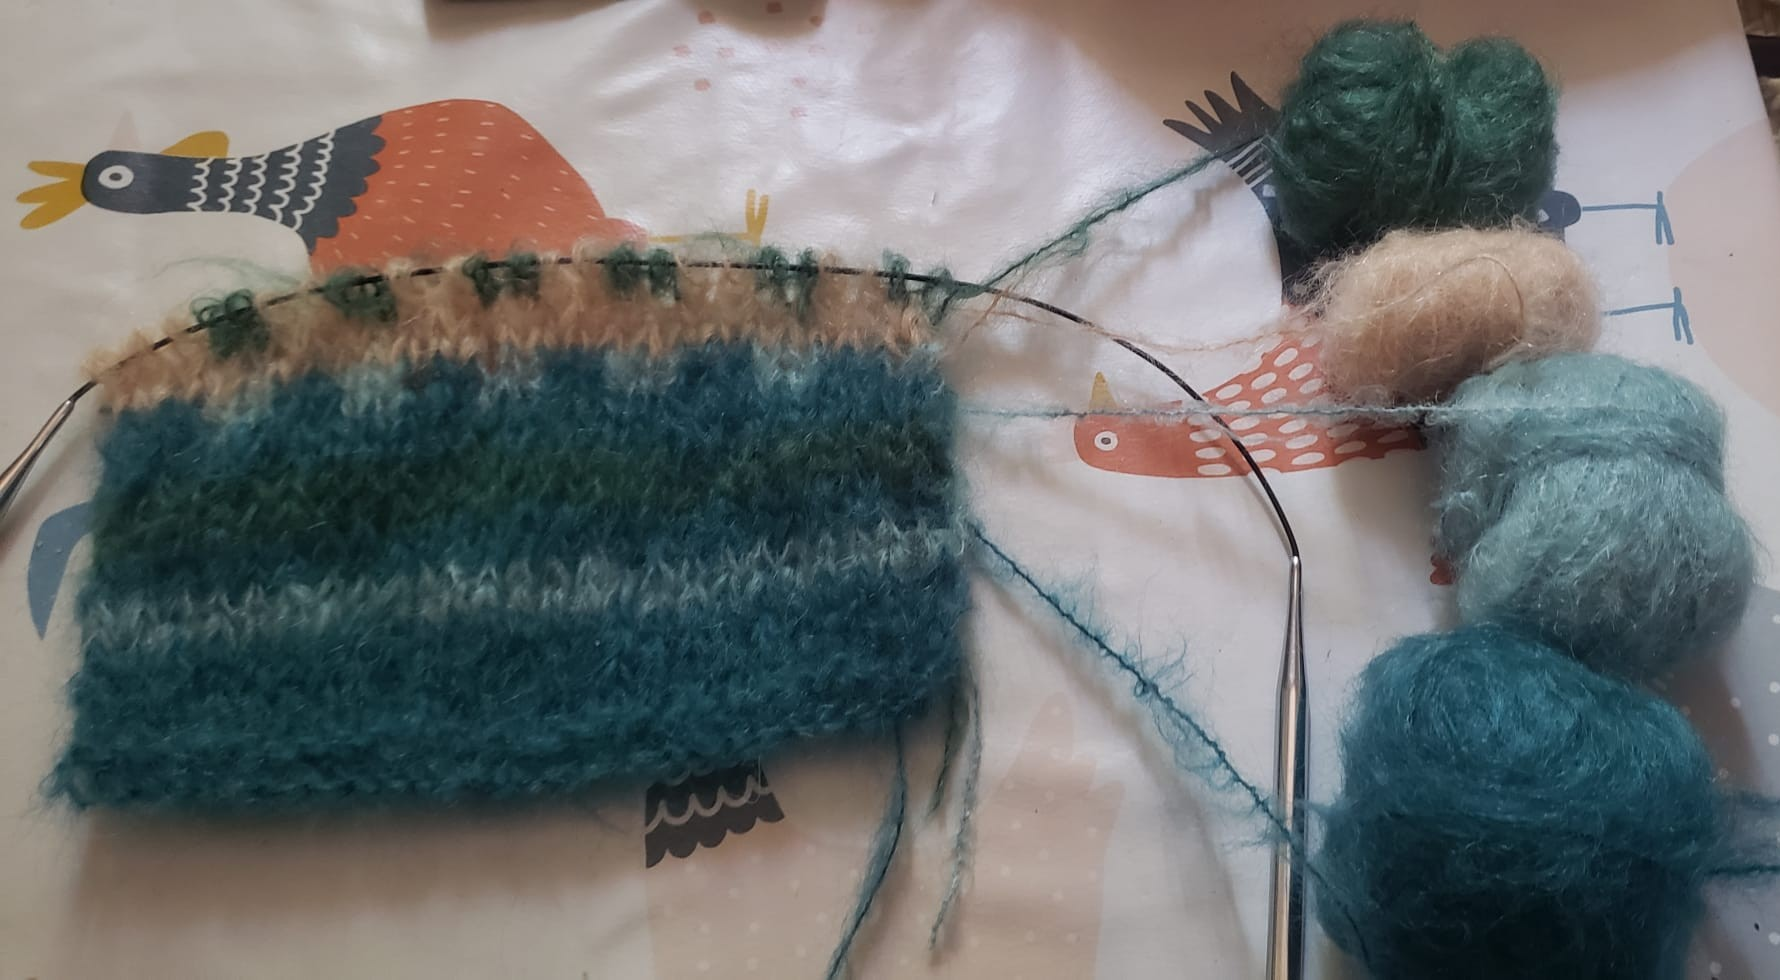
\includegraphics[width=.8\columnwidth]{aux/figures/knitting-example}};
		\draw[->] ($(fig.south west) + (-.1, -.1)$) -- node[anchor=east] {\rotatebox{90}{Direction of Reduction}} ($(fig.north west) + (-.1, .1)$);
	\end{tikzpicture}
	\caption{Example of a \emph{Jacquard} knitwork. Photography and work courtesy
		of the author's mother.}
	\label{fig:knitting-example}
\end{figure}

The other reason being the tangible interpretation of how things work
underlying the idea of a string diagram:
Suppose you're knitting a rainbow scarf.
You have multiple threads (the different words) of the different colours (their
types and effects) you're using to knit the scarf.
When you decide to change the color you take the different threads you have
been using, and mix them up:
You can create a new colour\footnote{I know this is not how wool works, but
	if you prefer you can imagine a pointillist-like way of drawing using multiple
	coloured lines that superimpose on each other, or a marching band's multiple
	instruments playing either in harmony or in disharmony and changing that
	during a score.} thread from two (that's the base combinators) create a
thicker one from two of the same colour (the applicative mode and the monadic
join), put aside a thread until a later step (that's the $\fmap$), add a new
thread to the pattern (that's the unit), or cut a thread you will not be
using anymore (that's the co-units and closure operators).
Changing a thread by cutting it and making a knot at another point is basically
what the eject combinators do.
This more tangible representation can be seen in a larger diagram in Figure
\ref{fig:3dparsing-diagram}.
The sections in the rectangle represent what happen when considering our
combination step as implementing patterns inside a knitwork, as seen in Figure
\ref{fig:knitting-example}.
The different patterns provide, in order, a visual representation of the
different ways one can combine two strings, i.e., two types and thus two
denotations.
The sections outside of the rectangle are the strings of yarn not currently
being used to make a pattern.

\begin{figure*}
	\centering
	% \def\shear#1#2{
	\begin{scope}[cm={1, 0, #1, (0, 0)}]
		#2
	\end{scope}
}
\def\rt#1{\rotatebox{180}{#1}}

\newcommand{\wool}[1][]{\draw[decorate, decoration={random steps, amplitude=1pt, segment length=1pt}, #1]}

\colorlet{cif}{blue}
\colorlet{ceve}{red}
\colorlet{cpass}{yulm}
\colorlet{crain}{vulm}
\colorlet{cevepass}{ceve!50!cpass}
\colorlet{cifevp}{cevepass!50!cif}
\colorlet{cend}{cifevp!50!crain}

\def\theopac{.2}

\tikzset{
	pics/pelote/.style args={#1}{
			code = {
					\coordinate (-center) at (0,0);
					\draw (-center) ellipse (1cm and .7cm);
					\foreach \i in {1,...,25}{
							\pgfmathsetmacro{\gdaxe}{.1 + .9 * \i/25}
							\pgfmathsetmacro{\ptaxe}{.1 + .6 * \i/25}
							\draw[#1] (-center) ellipse (\gdaxe cm and \ptaxe cm);
						}
					\draw ($(-center) + (0, 0)$) ellipse (.1cm and .1cm);
					\coordinate (-north) at ($(-center) + (0, .7cm)$);
					\coordinate (-south) at ($(-center) + (0, -.7cm)$);
					\coordinate (-west) at ($(-center) + (-1cm, 0)$);
					\coordinate (-east) at ($(-center) + (1cm, 0)$);
				}
		}
}

\tikzset{%
main3D/.pic={%
\shear{.2, .7}{\pic[transform shape] (w1) at (0, 0) {pelote=cif};}
\shear{.2, .8}{\pic[transform shape] (w2) at ($(w1-east) + (1.5cm, .3)$) {pelote=ceve};}
\shear{.2, 1}{\pic[transform shape] (w3) at ($(w2-east) + (1.5cm, -.2)$) {pelote=cpass};}
\shear{.2, .9}{\pic[transform shape] (w4) at ($(w3-east) + (1.5cm, -.1)$) {pelote=crain};}
\node[anchor=south] (w2-word) at (w2-north) {\rt{\vphantom{pb}\textbf{everyone}}};
\path let
\p1 = (w1-north),
\p2 = (w2-word),
\p3 = (w3-north),
\p4 = (w4-north)
in
coordinate[label=center:\vphantom{pb}\textbf{if}] (w1-word) at (\x1, \y2)
coordinate[label=center:\vphantom{pb}\textbf{passed}] (w3-word) at (\x3, \y2)
coordinate[label=center:\vphantom{pb}\textbf{it rained}] (w4-word) at (\x4, \y2);
\path let
\p1 = ($(w1-word.north) + (0, .7)$),
\p2 = (w2-word),
\p3 = (w3-word),
\p4 = (w4-word)
in
coordinate[label=center:$\vphantom{pb}\lambda c. \forall x. c\, x$] (w2-denot) at (\x2, \y1)
coordinate[label=center:$\vphantom{pb}\w{pass}$] (w3-denot) at (\x3, \y1)
coordinate[label=center:$\vphantom{pb}\w{rain}$] (w4-denot) at (\x4, \y1)
;
\coordinate (base) at (0, -2);
%
\wool[cif] let \p1 = (base),	\p2 = (w1-south) in	(\x2, \y2) -- (\x2, \y1) coordinate[black, label=right:$\t \to \t \to \t$] (if) ;
\wool[ceve] let \p1 = (base),	\p2 = ($(w2-south) + (+.3, .02)$) in	(\x2, \y2) -- (\x2, \y1) coordinate[black, label=left:$\f{C}$] (everyone-t);
\wool[ceve] let \p1 = (base),	\p2 = ($(w2-south) + (-.2, .011)$) in	(\x2, \y2) -- (\x2, \y1) coordinate[black, label=right:$\e$] (everyone-f);
\wool[cpass] let \p1 = (base),	\p2 = (w3-south) in	(\x2, \y2) -- (\x2, \y1) coordinate[black, label=left:$\e \to \t$] (passed);
\wool[crain] let \p1 = (base),	\p2 = (w4-south) in	(\x2, \y2) -- (\x2, \y1) coordinate[black, label=left:$\t$] (rain);
%
\wool[cif, opacity=\theopac] (if) -- +(0, -9.5) coordinate (ifp2);
%
%
%
\coordinate (evef1) at ($(everyone-f) + (-.5, -2)$);
\coordinate (evet1) at ($(everyone-t) + (-1, -2.5)$);
\path let
\p1 = (evef1),
\p2 = ($(passed) + (0, -3.5)$)
in coordinate (pass1) at (\x1, \y2);
\draw[opacity=\theopac, ceve] (everyone-f) -- ++(0, -1.5) to[out=-90, in=0] (evef1) -- ++(-3, 0) coordinate (eveftmp) (everyone-t) -- ++(0, -1.5) to[out=-90, in=0] (evet1) -- ++(-3, 0) coordinate (evettmp);
\draw[opacity=1, ceve] (evettmp) -- +(-1.5, 0) coordinate (evet2) (eveftmp) -- +(-1.5, 0) coordinate (evef2);
\draw[opacity=\theopac, cpass] (passed) -- ++(0, -1.5) to[out=-90, in=0] (pass1) -- ++(-3, 0) coordinate (passtmp);
\draw[opacity=1, cpass] (passtmp) -- +(-.5, 0) coordinate (pass2);
\coordinate (evef3) at ($(evef2) + (-2, -2)$);
\coordinate (evet3) at ($(evet2) + (-1.5, -1.5)$);
\coordinate (pass3) at ($(pass2) + (-.5, -.5)$);
\draw[ceve] (evef2) to[out=180, in=90] (evef3) (evet2) to[out=180, in=90] (evet3);
\draw[cpass] (pass2) to[out=180, in=90] (pass3);
%
\node[circle, draw=black] (eve-pass-fmap) at ($($(evet3)!.5!(pass3)$) + (0, -1.5)$) {\rt{$\combML_{\f{C}}$}};
\draw[ceve] (evef3) to[out=-90, in=160] (eve-pass-fmap);
\draw[ceve] (evet3) to[out=-90, in=160] (eve-pass-fmap);
\draw[cpass] (pass3) to[out=-90, in=20] (eve-pass-fmap);
\node[circle, draw=black] (eve-pass-app) at ($(eve-pass-fmap) + (0, -2)$) {\rt{$<$}};
\draw[ceve] (eve-pass-fmap) to[out=200, in=160] (eve-pass-app);
\draw[cpass] (eve-pass-fmap) to[out=-20, in=20] (eve-pass-app);
\node[anchor=west] at (eve-pass-app.east) {\rt{\vphantom{pb}$\e$}};
\node[anchor=east] at (eve-pass-app.west) {                 \rt{\vphantom{pb}$\e \to \t$}};
\wool[cevepass] (eve-pass-app) to[out=-90, in=180] ++(1, -1) -- ++(1, 0) coordinate (evpaptmp2);
\wool[cevepass, opacity=\theopac] (evpaptmp2) -- ++(3.5,0) to[out=0, in=90] +(1, -1) coordinate[label=above right:$\t$] (eve-pass-t);
\draw[black] let
\p1 = ($(evpaptmp2) + (0, -.5)$),
\p2 = ($(evef2) + (-3.5, .5)$)
in
(\x1, \y1) rectangle (\x2, \y2);
%
\wool[cevepass] let
\p1 = (evpaptmp2),
\p2 = (eve-pass-fmap.east) in
(eve-pass-fmap.east) -- (\x1, \y2) coordinate (evpaptmp);
\wool[cevepass, opacity=\theopac] (evpaptmp) -- ++(4, 0) to[out=0, in=90] ++(1, -1) -- +(0, -3) coordinate[label=above left:$\f{C}$] (eve-pass-f);
%
%
%
%
\draw[opacity=\theopac, cif] let
\p1 = (evpaptmp2),
\p2 = ($(ifp2) + (0, -1)$) in
(ifp2) to[out=-90, in=0] ++(-1, -1) -- (\x1, \y2) coordinate (if2) ;
\draw[opacity=\theopac, cevepass] let
\p1 = (if2),
\p2 = ($(eve-pass-t) + (0, -2)$),
\p3 = ($(eve-pass-f) + (0, -2.5)$) in
(eve-pass-t) -- ++ (0, -1) to[out=-90, in=0] ++(-1, -1) -- (\x1, \y2) coordinate (eve-pass-t2)
(eve-pass-f) -- ++ (0, -1) to[out=-90, in=0] ++(-1.5, -1.5) -- (\x1, \y3) coordinate (eve-pass-f2);
%
\draw[cif] (if2) -- ++(-2, 0) to[out=180, in=90] ++(-1, -1) -- +(0, -1.5) coordinate (if3);
\draw[cevepass] (eve-pass-t2) to[out=180, in=90] +(-1, -1) coordinate (eve-pass-t3);
\draw[cevepass] (eve-pass-f2) to[out=180, in=90] +(-.5, -.5) coordinate (eve-pass-f3);
%
\node[circle, draw=black] (if-evp-dn) at ($($(if3)!.5!(eve-pass-t3)$) + (0, -1)$) {\rt{$\combDN_{\Downarrow}$}};
\draw[cevepass] (eve-pass-f3) to[out=-90, in=20] (if-evp-dn) (eve-pass-t3) to[out=-90, in=20] (if-evp-dn);
\draw[cif] (if3) to[out=-90, in=160] (if-evp-dn);
\node[circle, draw=black] (if-evp-app) at ($(if-evp-dn) + (0, -2)$) {\rt{$>$}};
\draw[cif] (if-evp-dn) to[out=200, in=160] (if-evp-app);
\draw[cevepass] (if-evp-dn) to[out=-20, in=20] (if-evp-app);
\node[anchor=west] at (if-evp-app.east) {\rt{\vphantom{pb}$\t$}};
\node[anchor=east] at (if-evp-app.west) {\rt{\vphantom{pb}$\t\to\t\to\t$}};
%
\wool[cifevp] (if-evp-app) to[out=-90, in=180] ++(1, -1) -- ++(1, 0) coordinate (ifevptmp);
\wool[cifevp, opacity=\theopac] (ifevptmp) -- ++(3.5,0) to[out=0, in=90] +(1, -1) coordinate[label=left:$\t \to \t$] (if-evp-t);
\draw[black] let
\p1 = ($(ifevptmp) + (0, -.5)$),
\p2 = ($(if2) + (-5, .5)$)
in
(\x1, \y1) rectangle (\x2, \y2);
\wool[crain, opacity=\theopac] let \p1 = (if-evp-t), \p2 = (rain) in (rain) -- (\x2, \y1) coordinate (rainp2);
%
%
%
%
\draw[opacity=\theopac, cifevp] (if-evp-t) to[out=-90, in=0] ++(-1, -1) -- +(-3.5, 0) coordinate (if-evp-t2);
\draw[opacity=\theopac, crain] let
\p1 = (if-evp-t2),
\p2 = ($(rainp2) + (0, -2)$) in
(rainp2) to[out=-90, in=0] ++ (-2, -2) -- (\x1, \y2) coordinate(rain2);
\draw[cifevp] (if-evp-t2) -- ++(-2, 0) to[out=180, in=90] ++(-1, -1) -- +(0, -1) coordinate (if-evp-t3);
\draw[crain] (rain2) to[out=180, in=90] +(-1, -1) coordinate (rain3);
\node[circle, draw=black] (ifrain) at ($($(if-evp-t3)!.5!(rain3)$) + (0, -1)$) {\rt{$>$}};
\draw[cifevp] (if-evp-t3) to[out=-90, in=160] (ifrain);
\draw[cif] (rain3) to[out=-90, in=20] (ifrain);
\wool[cend] (ifrain) to[out=-90, in=180] ++(1, -1) -- ++(1, 0) coordinate (ifrain2);
\draw[black] let
\p1 = ($(ifrain2) + (0, -.5)$),
\p2 = ($(if-evp-t2) + (-5, .5)$)
in
(\x1, \y1) rectangle (\x2, \y2);
\wool[opacity=\theopac, cend] (ifrain2) -- ++(3.5, 0) to[out=0, in=90] ++(1, -1) to[out=-90, in=0] ++(-1, -1) -- ++(-3.5, 0) coordinate (sentence-t);
\wool[cend] (sentence-t) -- ++ (-1, 0) to[out=180, in=90] ++(-1, -1) coordinate[label=below right:$\t$] (end-before) -- +(0, -2) coordinate (end);
\draw[black] let \p1 = (sentence-t), \p2 = ($(end) + (0, 0)$) in ($(sentence-t) + (-5, .5)$) rectangle (\x1, \y2);
\draw[->] let
\p1 = ($(w4-east) + (1, -.2)$),
\p2 = ($(end) + (0, 1)$),
\p3 = ($(\x1, \y1)!.5!(\x1, \y2)$)
in (\x1, \y1) -- (\x1, \y2)
node[anchor=west] at (\x3, \y3) {\rotatebox{-90}{Direction of Reduction}};
}
}

\resizebox{\textwidth}{!}{%
	\rotatebox{180}{%
		\begin{tikzpicture}
			\pic[yscale=.6, every label/.style={rotate=180}] at (0, 0) {main3D};
		\end{tikzpicture}
	}
}


	\caption{3D-like Representation of the Diagrammatic Parsing of a Sentence. See \ref{fig:tree-rain} for the translation in a Parse Tree}
	\label{fig:3dparsing-diagram}
\end{figure*}

\subsubsection{The Coproduct Categorical Approach to Syntax}
\label{subsubsec:coprod}
% TODO: add a reference to Bella's paper explaining the interest of such 
% notions when talking about the syntax-semantic interface/
In this section based on the work by
\cite{marcollimatildeetchomskynoametberwickrobertc.MathematicalStructureSyntactic},
we explore the integration of our notion inside the structure of syntactic
merge, and why the two formalisms are compatible.
The idea behind that structure is to see the union of trees as a product and
the merging of trees as based on a coproduct in a well-defined Hopf algebra.
Now of course, with our insights on syntactico-semantic parsing, we can either
think of our parsing structure labeled by multiple modes, as in
\cite{bumfordEffectdrivenInterpretationFunctors2025}, or think of it as string
diagrams, as presented above.
In both cases, we make a more or less implicit use of the merge operation.

\medskip

Labeled trees can be seen as computed from a sequence of labeled merge.
As such, it is easy to see how one can adapt the construction of a purely
syntactic merge onto a semantic merge, using a similar approach.
There is just the need for a coloured operad to create a series of labeled
merges, like proposed in \cite{melliesCategoricalContoursChomskySchutzenberger2025}
for example.
Since there is a one-to-one mapping from our string diagrams to parse trees,
mapping explained when comparing the tables for denotations of combinators
in Figure \ref{fig:combinator-denotations} and Figure 12 in
\cite{bumfordEffectdrivenInterpretationFunctors2025}, or by looking at the
parse trees equivalent to string diagrams in Figures \ref{fig:parsing-diagram},
\ref{fig:parsing-diagram2} and \ref{fig:3dparsing-diagram}, it is easy to see
that indeed, there is a notion of merge inside our diagrams that can in a way
be expressed through a Hopf algebra, by transporting the diagrams to and from
their equivalent parsing diagram.
More generally, what this means is that a merge, in our string diagrams, is
the addition of a combinator to one, two\footnote{Or more, see
	\ref{app:arities-and-denots}} without conditions.
This is useful as a definition, because it allows integration of our system in
a broader framework, including for example the notion of morphosyntactic trees.

\medskip

However, this is not fully satisfying: like for syntax trees, applying a random
sequence of merges to a set of input strings will not always yield a properly
typed denotation.
Since type soundness is the main feature of our system, it seems weird to have
a definition of merge which cannot take that into account.

\subsection{Rewriting Rules}
\label{subsec:rewrite}
Here we provide a rewriting system on derivation trees that allows us to
improve our time complexity by reducing the size of the disambigued grammar.
In the worst case, in big o notation there is no improvement in the size of the
sentence, but there is no loss.
The goal is to reduce branching in the definition of $PT$, as this will easily
translate into reductions in the grammar.

\medskip

When considering the grammar version of the semantic system, the reductions
written below cannot be done when using only one step at a time.
To get around this, a simple way might be to expand the size of the grammar to
consider reductions two at a time, by adding an intermediate non-terminal.
Then, while the size of the grammar becomes quadratic in
$\abs{\mFunc\left(\mL\right)}$, because this also reduces the number of
reductions needed to get the derivations, this compensates the increase, and
actually reduces the time complexity when the reducing the number of rules
after equivalence.
Obviously the same reasoning applies when considering reductions of length $3$,
$4$ and more.
We really just need to consider the same set of reductions that the one
proposed below.

\medskip

First, let's consider the reductions proposed in Section \ref{sec:nondet}.
Those define normal forms under Theorem \ref{thm:confluence} and thus we can
use those to reduce the number of trees.
Indeed, we usually want to reduce the number of effects by first using the
rules \emph{inside} the language, understand, the adjunction co-unit and
monadic join.
Thus, when we have a presupposition of the form:
\begin{equation*}
	\PT{\blank}{\cont x: \f{M}\f{M}\tau} \poulpe \text{or} \poulpe
	\PT{\blank}{\cont x: RL\tau}
\end{equation*}
we always simplify it directly, as not always doing it would propagate
multiple trees.
This in turn means we always verify the derivational rules we set up in the
previous section for the join equations of the monad.

\medskip

Secondly, while there is no way to reduce the branching proposed in the
previous section since they end in completely different reductions, there is
another case in which two different reductions arise:
\begin{equation*}
	\PT{\blank}{\cont x: \f{F}\tau_{1}} \poulpe \text{and} \poulpe
	\PT{\blank}{\cont y: \f{G}\tau_{2}}
\end{equation*}
Indeed, in that case we could either get a result with effects $\f{F}\f{G}$ or
with effects $\f{G}\f{F}$.
In general those effects are not the same, but if they happen to be, which
trivially will be the case when one of the effects is external, the plural or
islands functors for example.
When the two functors commute, the order of application does not matter and
thus we choose to get the outer effect the one of the left side of the
combinator.

\medskip

Thirdly, there are modes that clearly encompass other ones\footnote{Here we use
	the grammar notation for ease of explanation}.
One should not use mode $\combUR$ when using $\combMR$ or $\combDN \combMR$
and the same goes for the left side, because the two derivations yield simpler
results.
Same things can be said for certain other derivations containing the lowering
and co-unit combinators.

\noindent We use $\combDN$ when we have not used any of the following, in all
derivations:
\begin{multicols}{2}
	\begin{itemize}
		\item $m_{\f{F}}, \combDN, m_{\f{F}}$ where
		      $m \in \{\combMR, \combML\}$
		\item $\combML_{\f{F}}, \combDN, \combMR_{\f{F}}$
		\item $\combA_{\f{F}}, \combDN, \combMR_{\f{F}}$
		\item $\combML_{\f{F}}, \combDN, \combA_{\f{F}}$
		\item $\combC$
	\end{itemize}
\end{multicols}
\noindent We use $\combJ$ if we have not used any of the following,
for $j \in \{\epsilon, \combJ_{\f{F}}\}$
\begin{multicols}{2}
	\begin{itemize}
		\item $\left\{m_{\f{F}}, j, m_{\f{F}}\right\}$ where
		      $m \in \{\combMR, \combML\}$
		\item $\combML_{\f{F}}, j, \combMR_{\f{f}}$
		\item $\combA_{\f{F}}, j, \combMR_{\f{F}}$,
		\item $\combML_{\f{F}}, j, \combA_{\f{F}}$
		\item $k, \combC$ for $k \in \{\epsilon, \combA_{\f{F}}\}$
		\item If $\f{F}$ is commutative as a monad:
		      \begin{itemize}
			      \item $\combMR_{\f{F}}, \combA_{\f{F}}$
			      \item $\combA_{\f{F}}, \combML_{\f{F}}$
			      \item $\combMR_{\f{F}}, j, \combML_{\f{F}}$
			      \item $\combA_{\f{F}}, j, \combA_{\f{F}}$
		      \end{itemize}
	\end{itemize}
\end{multicols}

\begin{theorem}
	The rules proposed above yield equivalent results.
\end{theorem}
\begin{proof}
	For the first point, the equivalence has already been proved under Theorem
	\ref{thm:confluence}.
	For the second point, it is obvious since based on an equality.
	For the third point, it's a bit more complicated.
	The rules about not using combinators $\combUL$ and $\combUR$ come from the
	notion of handling and granting termination and decidability to our system.
	The rules about adding $\combJ$ and $\combDN$ after moving two of the same
	effect from the same side (i.e. $\combML \combML$ or $\combMR\combMR$) are
	normalization of a the elevator equations \ref{eq:elevator}.
	Indeed, in the denotation, the only reason to keep two of the same effects
	and not join them\footnote{Provided they can be joined.} is to at some point
	have something get in between the two.
	Joining and cloture should then be done at earliest point in parsing where it
	can be done, and that is equivalent to later points because of the elevator
	equations, or Theorem \ref{thm:isotopy}.
	The last set of rules follows from the following: we should not use $\combJ
		\combML \combMR$ instead of $\combA$, as those are equivalent because of the
	equation defining them.
	The same thing goes for the other two, as we should use the units of monads
	over applicative rules and fmap.
\end{proof}

\medskip

The observant reader might have noticed that this is simply a scheme to apply
typing rules to a syntactic derivation, but that this will not be enough to
actually gain all reductions possible in polynomial time.
This is actually not feasible (because of the intrinsic ambiguity of the
English language, as proved for example by the sentence \emph{The man sees the
	girl using a telescope}).
Even then, we are far from reducing to a minimum the number of different paths
possible to get a same final denotation.
This can only happen once a confluent reduction scheme is provided for the
denotations.
When this is done, we can combine the reduction schemes for effects along with
the one for denotation and the one for combinations in one large reduction
scheme.
Indeed, trivally, the tensor product of confluent reduction schemes forms a
confluent reduction scheme, whose maximal reduction length is the sum of the
maximal reduction lengths\footnote{Actually it is at most that, but that does
	not	really matter.}.

\medskip

When using our diagrammatic approach to parsing, which, again, is just a
rewriting in a more graphical fashion of our typing rules and our CFG-like
rules, we can write all the reductions described above to our paradigm:
it simply amounts to constructing a set of normal forms for the string diagrams.
This leads to the same algorithms developed in Section \ref{sec:nondet} being
usable here: we just have a new improved version of Theorem
\ref{thm:confluence} which adds the normal forms specified in this section to
the newly added \emph{orthogonal} axis of diagrammatic computations.
What we're actually doing is computing two different normal forms along the
tensor product of our reduction schemes\footnote{Just like we already have (or
	should have) a tensor scheme for the denotations and combination modes.},
but again, that only amounts to computing a larger normal form.
Moreover, considering the possible normal forms of syntactic reductions simply
adds another way to reduce our diagrams to normal forms.
Since all of these forms can be attained in polynomial time, it is clear that
finding a normal-form diagram, which is exactly a normal-form denotation for
the sentence, is doable in polynomial time\footnote{Of course, this is only
	true when the denotations can be normalized in polynomial time.}

\medskip

Once again, there is no evidence that our system is complete, if not the
contrary, so the arguments developed in Section \ref{subsubsec:sanity} are
still valid.
A way to "complete" it, although it would still probably be incomplete would be
to write an automatized prover in Lean, but this is out of the scope of this
project, as it would not do many improvements.
